% !TeX spellcheck = pt_BR
\chapter{Redes Bayesianas}%
Uma \gls{bn} provê uma representação compacta de distribuições de probabilidades grandes demais para lidar usando especificações tradicionais e provê um método sistemático e localizado para incorporar informação probabilística sobre uma dada situação.

Uma BN é um grafo acíclico direcionado (DAG) que representa uma função de distribuição de probabilidades conjunta de variáveis que modelam certo domínio de conhecimento. Ela é constituída de uma DAG, de variáveis aleatórias (também chamadas de nós da rede), arcos direcionados da variável pai para a variável filha e uma tabela de probabilidades condicionais (CPT) associada a cada variável.
\begin{figure}[H]
	\centering
	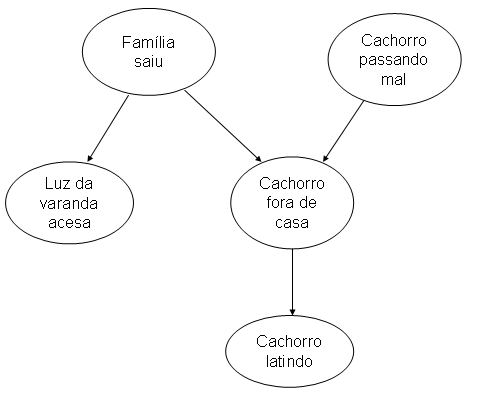
\includegraphics[width = 300px]{figuras/BN1}
	\caption[extraída do artigo do Laecio]{Exemplo family-out}
	\label{fig:familyBN}
\end{figure}

Nesse exemplo, suponhamos que se queira determinar se a família está em casa ou se ela saiu. Pelo grafo, pdoemos perceber que o fato de a luz da varanda estar acesa e de o cachorro estar fora de casa são indícios de que a família tenha saído. 

\section{Definição Formal}
Uma rede Bayesiana consiste em uma fatoração de uma distribuição de probabilidade e um DAG correspondente. Tais assertivas de independências condicionais podem ser inferidas diretamente da fatoração correspondente às 